\documentclass[pdf]{beamer}

\usepackage[utf8]{inputenc}
\usepackage[IL2]{fontenc}
\usepackage[slovak]{babel}
\usepackage{times}
\usetheme{berkeley}
\usecolortheme{dolphin}
\usepackage{textpos}
\usepackage{caption}
\usepackage{lipsum}
\captionsetup{font=scriptsize,labelfont=scriptsize}

\title{História kníhtlače}
\author{Anton Firc}
\institute{Vysoké učení technické v~Brně\\ Fakulta informačních technologií}
\date{\today}

\begin{document}
	
	\frame{
		\titlepage
	}
	
	\addtobeamertemplate{frametitle}{}{%
		\begin{textblock*}{100mm}(-0.18\textwidth,-1.25cm)
			
\includegraphics[height=1cm,width=1cm]{fit.png}
		\end{textblock*}}
	
	\frame{
		\frametitle{Prehľad}
		\tableofcontents	
	}
	
	\frame{
		\frametitle{Motivácia}
		\begin{itemize}
			\item 	Vynájdenie kníhtlače možno bez akýchkoľvek pochybností zaradiť medzi najvýznamnejšie udalosti celých dejín.
			
			\item Vynálezom kníhtlače sa začala nová epocha komunikačnej techniky. 
			
			\item Tento vynález umožnil mnohonásobné zvýšenie produkcie knihy. 
		\end{itemize}
	
		
		
	}
	
	\section{Vývoj písma}
	
	\frame{
		\frametitle{Počitaky}
		\begin{itemize}
			\item Už v~praveku sa ľudia pokúšali zaznamenať dôležité udalosti vo svojom živote kresbami.
			
			\item Prvé písmové sústavy sa vyvinuli nezávisle od seba v~Egypte, Babylone a v~Číne.
			
			\item Egypťania používali okolo roku 3000 p.n.l. úhľadné obrázkové písmo s~plnou kresbou tzv. hieroglify.
			
			\begin{figure}[h]
				\begin{center}
					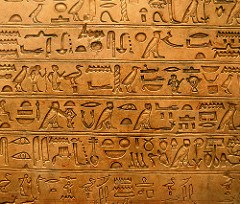
\includegraphics[width = 3cm]{hieroglyph.jpg}
					\caption{Hieroglyfy}
					\label{obr1}
				\end{center}	
			\end{figure}
			
		\end{itemize}
	}

	\frame{
		\frametitle{Počitaky}
		\begin{itemize}
			\item Najdôležitejším pokrokom v~dejinách písma bolo Fénické písmo vyvinuté okolo r. 1000 p.n.l.
			
			\item Vzniklo z~neho až 80\% známych abecedných sústav.
			
			\item Grécka abeceda predstavovala prvé dokonalé hláskové písmo v~dejinách.
			
			\item Z~Grécka sa do Európy rozšírilo románske písmo- latinka a staroslovanské písmo.
		\end{itemize}
	
		\begin{figure}[h]
			\begin{center}
				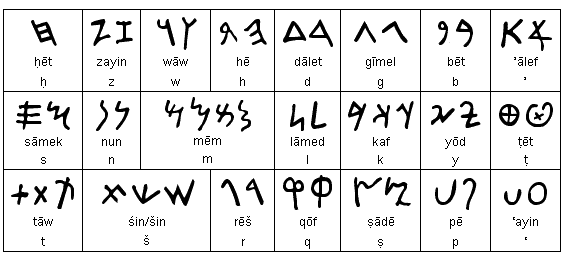
\includegraphics[width = 4cm]{phoenic.png}
				\caption{Fenické písmo}
				\label{obr2}
			\end{center}	
		\end{figure}
	}
	
	\section{Predchodcovia Knihy}
	
	\frame{
		\frametitle{Predchodcovia Knihy}
		\begin{itemize}
			\item<1-> \Large{\textsc{Hlinené tabuľky\\}} {\scriptsize drevené, olovené, alebo tabuľky vyrobené zo slonovej kosti.}
			\item<2-> \Large{\textsc{Zvitok a papyrus\\}} {\scriptsize zvitky sa vyrábali z~\emph{papyrusu} - papiera vyrobeného z~rastliny}
			\item<3-> \Large{\textsc{Kódex a pergamen\\}} {\scriptsize poskladané pergamenové papiere zopnuté dvomi drevenými tabuľkami}
			\item<4-> \Large{\textsc{Kniha a papier\\}} {\scriptsize kniha a papier skoro tak ako ich poznáme dnes}
		\end{itemize}
	}

	\section{Vznik kníhtlače}
	\frame{
		\frametitle{Vznik kníhtlače}
		\begin{itemize}
			\item Až do vynájdenia kníhtlače sa väčšina kníh písala ručne.
			
			\item Prvý pokus použiť izolované znaky k~zostaveniu sadzby urobil už v~roku 1004 nášho letopočtu Bi-Šeng.
			
			\item V~Európe sa ľudia začali zaoberať kníhtlačou až  na začiatku 15. storočia.
			
			\item Zároveň s~Gutenbergom prevádzali pokusy aj mnohí ďalší, napriek tomu je však ustálená predstava o~prvenstve Gutenberga.
		\end{itemize}
	}

	\subsection{Johan Gutenberg}

	\frame{
		\frametitle{Johan Gutenberg}
	\begin{columns}
		\column{0.6\linewidth}
			Johann Gutenberg sa narodil v~meste Mainz ako syn kupca Friela Gensfleischa. Ďalšie meno zum Gutenberg prijal jeho otec až neskôr podľa miesta, kde žili.Odborníci sa domnievajú že študoval na známej univerzite v~Erfurte. Po škole sa venoval výrobe zrkadiel a začal sa venovať aj kníhtlači. V~roku 1448 dostal pôžičku a zriadil svoju prvú tlačiareň. 
			
		
		\column{0.4\linewidth}
			\begin{figure}
				\begin{center}
					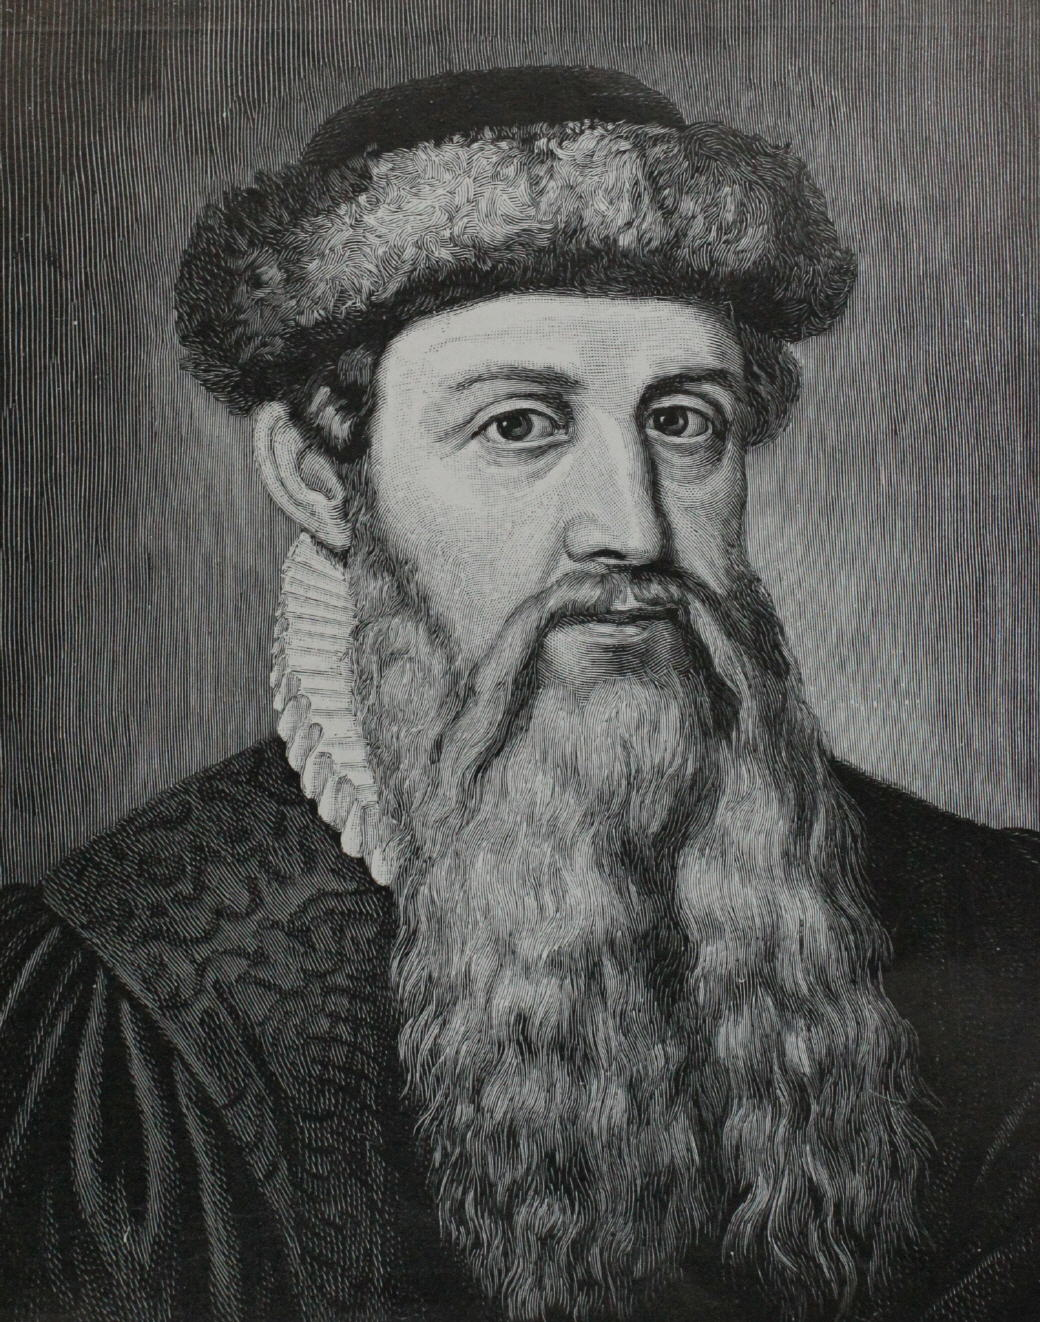
\includegraphics[width = 4cm]{Gutenberg.jpg}
					\caption{Johan Gutenberg}
					\label{obr3}
				\end{center}	
			\end{figure}
	\end{columns}
	}
	
	\frame{
		\frametitle{Johan Gutenberg}
		\begin{itemize}
			\item Gutenbergov hlavný vynález nebola kníhtlač, ale zostavenie strany z~jednotlivých písmen ktoré bolo možné preskupiť a znova použiť čo celú kníhtlač výrazne zlacnilo a zrýchlilo. 
			
			\item Aj keď Gutenberg sám so svojím objavom neprerazil, tento objav sa ukázal byť veľmi dôležitý, lebo odštartoval sériovú výrobu kníh a v~súvislosti s~tým informačnú a vedeckú revolúciu a rozšírenie vzdelanosti medzi širšie vrstvy.
		\end{itemize}
		
	}
	
	\section{Použité zdroje}
	
	\frame{
		\frametitle{Použité zdroje}
		
		\begin{thebibliography}{99}
			\bibitem{papyrus} Wikipédia - Kníhtlač [online] 29.3.2017 [cit. 20.4.2017] URL: \url{https://sk.wikipedia.org/wiki/Kn\%C3\%ADhtla\%C4\%8D}
			
			\bibitem{papyrus} Wikipédia - Papyrus [online] 24.10.2016 [cit. 20.4.2017] URL: \url{https://sk.wikipedia.org/wiki/Papyrus_(v\%C3\%BDrobok)} 
			
			\bibitem{papyrus} Wikipédia - Johan Gutenberg [online] 9.4.2017 [cit. 20.4.2017] URL: \url{https://sk.wikipedia.org/wiki/Johann_Gutenberg} 
			
			\bibitem{papyrus} Vznik a vývoj kníhtlače [online] 14.1.2006 [cit. 20.4.2017] URL: \url{http://referaty.aktuality.sk/vznik-a-vyvoj-knihtlace/referat-5123}
			
		\end{thebibliography}
		
	}

	\frame{
		\frametitle{Použité zdroje}
		
		\begin{thebibliography}{99}
			\bibitem{obr1} Obrázok \ref{obr1} : Hieroglyfy. Skopírované z~\url{https://flic.kr/p/7Hxa8g}
			
			\bibitem{obr2} Obrázok \ref{obr2} : Fenické písmo. Skopírované z~\url{https://flic.kr/p/633c1g}
			
			\bibitem{obr3} Obrázok \ref{obr3} : Johan Gutenberg. Skopírované z~
			\url{https://commons.wikimedia.org/w/index.php?curid=31396}
		\end{thebibliography}
	}
	
	
\end{document}